Neste capítulo é apresentado os conceitos do que é RAID e quais são as peculiaridades de suas principais categorias. O capítulo está dividido em duas seções, na primeira são apresentados os conceitos de RAID separado em subseções para os tipos RAID 0, RAID 1, RAID 2, RAID 3, RAID 4, RAID 5, RAID 6 e RAID 50. Finalmente, o capítulo termina com a seção de conclusões do capítulo.

%	\section{RAID}
		\section{Conceitos}
		O desempenho da unidade de processamento e da memória principal cresceu rapidamente. Para se ter uma ideia do tamanho do crescimento de desempenho destes componentes, entre os anos de 1974 e 1984 o desempenho deles aumentava em 40\% por ano.
		Deste modo uma instrução de CPU que realiza uma E/S(entrada/saída) para acessar um disco tem a possibilidade de se tornar um grande gargalo, devido ao fato de que o dispositivo de armazenamento magnético, em questão de velocidade de acesso, não acompanha o crescimento dos dois componentes principais, o processador e a memória.\\
		
		O RAID(originalmente a sigla do \textit{redundant array of inexpensive disk}, mas atualmente é mais conhecido como \textit{redundant array of independent disk}) se baseia no uso de disco extra para a recuperação da informação original em caso de uma falha num disco. Em ~\cite{patterson88} Patterson \textit{et al} demonstrou que sem um controle de tolerância à falhas, grandes \textit{arrays} de discos baratos não podem ser considerados úteis devido a sua baixa taxa de confiabilidade. A proposta inicial de Patterson \textit{et al} ao desenvolver o RAID era de que para superar o obstaculo da falta de confiabilidade era necessário o uso de discos extras que possuíssem informação redundante que possibilitassem a recuperação total das informações originais no caso da falha de algum disco. Vale ressaltar que a proposta inicial do RAID foi desenvolvida utilizando como referencia o \textit{hardware}, contudo, Petterson em seu artigo original ~\cite{patterson88} frisa que as ideias centrais do projeto poderiam ser aplicadas facilmente na implementação de \textit{softwares}, e este ponto é de fundamental importância para nosso trabalho. Sendo que a ideia central apresentada por Patterson era de quebrar os \textit{arrays} em grupos confiáveis, onde cada grupo possua discos extras possuidores de informação redundante que seriam utilizados para manter a previamente citada confiabilidade dos grupos. De forma que quando um disco falhar, em um espaço curto de tempo o disco faltoso será substituído por um novo disco e a informação que estava contida no antigo disco será totalmente reconstruída no novo utilizando as informações redundantes contida no grupo. Este tempo de espera ficou conhecido como \textit{mean time to repair (MTTR)} ou em uma tradução livre, "tempo de conserto". O MTTP pode ser reduzido se o sistema possuir discos extras que funcionem como peças sobressalentes em estado de prontidão de forma que quando um disco falha, ele é trocado por um desses discos extras de forma eletrônica, sem que haja a necessidade de intervenção humana (bastando apenas que de tempos em tempos, um técnico humano troque os discos defeituosos por novos discos extras). Patterson, ao desenvolver o conceito de RAID, assumiu que as falhas de discos são independentes e exponenciais. \\
		
		O RAID é separado em diferentes níveis, sendo que cada nível possuiu seus objetivos distintos e características intrínsecas. Os principais níveis de RAID serão apresentados e explicados nas próximas subseções deste trabalho.
		\\
		
		\subsection{RAID 0}
		
		Também conhecido como \textit{Strinping} ou fracionamento, pois os dados são fracionados igualmente entre dois ou mais discos, sem a preocupação com informação de paridade, tolerância a falhas ou redundância. Devido ao fato da completa falta de tolerância a falhas no RAID 0, a perda de um disco acarreta na perda (sem qualquer chance de recuperação) de todos os dados contidos no disco e da inutilização de todas as outras frações dos dados que estavam armazenadas nos outros discos do vetor, visto que estes arquivos jamais serão completamente recuperados.
		\\
		
		Por esta razão que o RAID 0 é usado apenas nos casos em que se deseja aumentar o desempenho do sistema ou como forma de criar uma grande unidade lógica de armazenamento utilizando-se dois ou vários discos físicos. Inclusive, é possível modelar um sistema em RAID 0 utilizando-se discos de diferentes capacidades, entretanto, é importante frisar que os discos com maior quantidade de armazenamento disponível serão limitados ao espaço máximo do menor disco do vetor, por exemplo, em um vetor montado com dois discos, um com 500GB e um segundo de 280GB possuirá o total de 560GB de armazenamento, ou seja, 280 X 2, nitidamente o disco de 500GB está sendo subutilizado neste vetor. \\
		
		A figura ~\ref{fig:raid0} representa o diagrama de um vetor modelado com o RAID 0 utilizando-se dois discos. Visto que os dados contidos nos discos 0 e 1 podem ser recuperados simultaneamente resulta na ilusão de que o \textit{drive} é mais rápido.\\
		
		\begin{figure}[htb]
			\begin{center}
				
				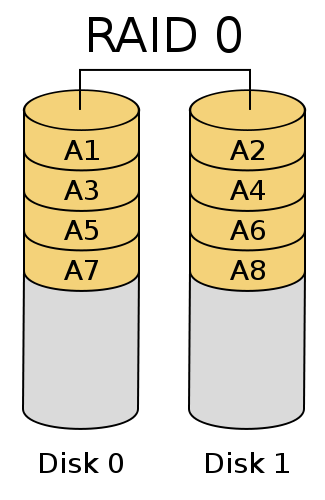
\includegraphics[clip,width=6.0cm]{images/RAID_0.png}
				\caption{Diagrama do RAID 0. }
				\label{fig:raid0}
			\end{center}
		\end{figure} 
		
		\subsubsection{Desempenho}
		
		RAID 0 pode ser usado em áreas onde o desempenho é crucial enquanto que a integridade dos dados é de pouca relevância, como ocorre no caso dos sistemas de jogos de video game online.\\
		
		\subsection{RAID 1}
		
		RAID 1 é também conhecido como \textit{mirror} ou espelhamento, visto que este nível consiste de uma copia exata de um conjunto de dados espalhado por dois ou mais discos. A configuração do RAID 1 não proporciona paridade ou fracionamento de dados, visto que os dados são apenas espelhados dentro de todos os discos pertencentes do vetor de discos, sendo que o espaço de armazenamento do vetor não pode ser maior do que o disco membro com o menor espaço de armazenamento. O vetor continuará funcional enquanto ao menos um membro do vetor esteja disponível. Esta configuração é útil para sistemas onde a confiança e desempenho de leitura é mais importante do que performasse de escrita ou um armazenamento eficiente. \\
		
		A figura ~\ref{fig:raid1} representa o diagrama de um vetor modelado com o RAID 1 utilizando-se dois discos.\\
		
		\begin{figure}[htb]
			\begin{center}
				
				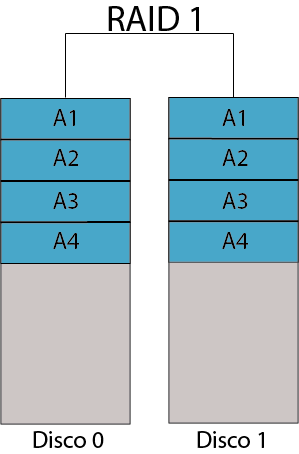
\includegraphics[clip,width=6.0cm]{images/RAID_1.png}
				\caption{Diagrama do RAID 1. }
				\label{fig:raid1}
			\end{center}
		\end{figure} 
		
		\subsubsection{Desempenho}
		
		Qualquer solicitação pode ser atendida por qualquer \textit{drive} no vetor. Sendo que no caso de solicitações de escrita o desempenho é comprometido pois é necessário que ela ocorra em todos os discos membros do vetor. \\
		
		\subsection{RAID 2}
		
		A configuração RAID 2 fraciona o dado ao nível do \textit{bit} ao invés de blocos, além de utilizar a técnica do Código de Hamming para a correção de erros. O eixo de rotação de todos os discos são sincronizados e o dado é fracionado de forma que cada sequência de \textit{bits} são armazenadas em discos diferentes. A paridade do código de hamming é calculada sobre os \textit{bits} correspondentes e armazenadas em ao menos um disco de paridade.\\
		
		A figura ~\ref{fig:raid2} representa o diagrama de um vetor modelado com o RAID 2 utilizando-se sete discos, sendo três deles utilizados como discos de paridade.\\
		
		\begin{figure}[htb]
			\begin{center}
				
				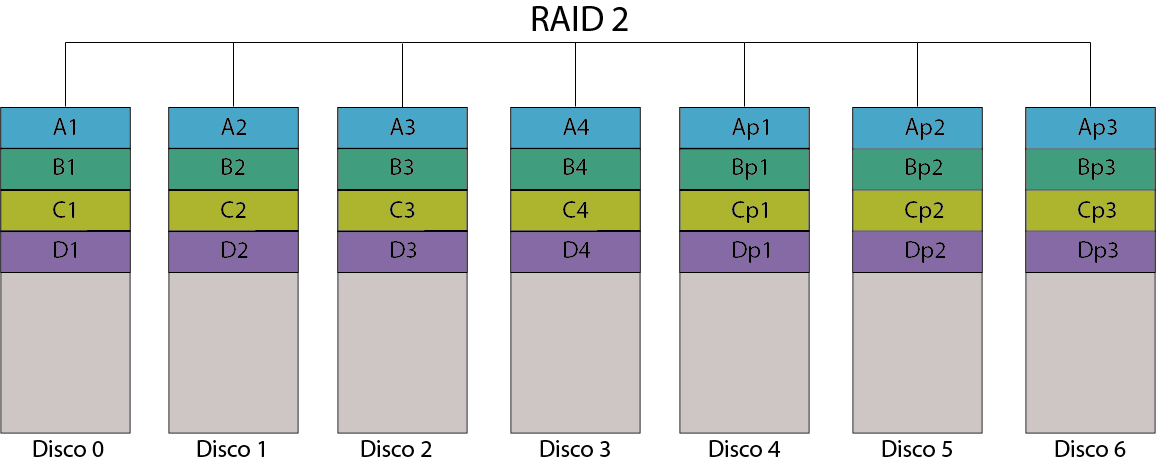
\includegraphics[clip,width=10.0cm]{images/RAID_2.png}
				\caption{Diagrama do RAID 2. }
				\label{fig:raid2}
			\end{center}
		\end{figure} 
		
		\subsubsection{Desempenho}
		Por utilizar o código de Hamming, possui forte tolerância a falhas. Entretanto, como os discos rígidos atualmente possuem correção interna de erros, o RAID 2 acabou perdendo seu propósito. 
	
	
		\subsection{RAID 3}
		
		Diferente do RAID 2, o RAID 3 fraciona os dados ao nível do \textit{byte}, tendo um disco dedicado de paridade. O eixo de rotação de todos os discos são sincronizados e o dado é fracionado de forma que cada sequência de \textit{bytes} são armazenadas em discos diferentes. A paridade é calculada sobre os \textit{bytes} correspondentes e armazenadas no disco de paridade. Apesar de existir casos de implementação, o RAID 3 dificilmente é utilizado na prática devida a forma de 
		fracionar os dados, onde a fração ao nível de \textit{bytes} é menos eficiente que a fração em nível de blocos que vai ser mostrado posteriormente.\\
		
		A figura ~\ref{fig:raid3} representa o diagrama de um vetor modelado com o RAID 3 utilizando-se quatro discos, sendo um deles utilizados como disco de paridade.\\
		
		\begin{figure}[htb]
			\begin{center}
				
				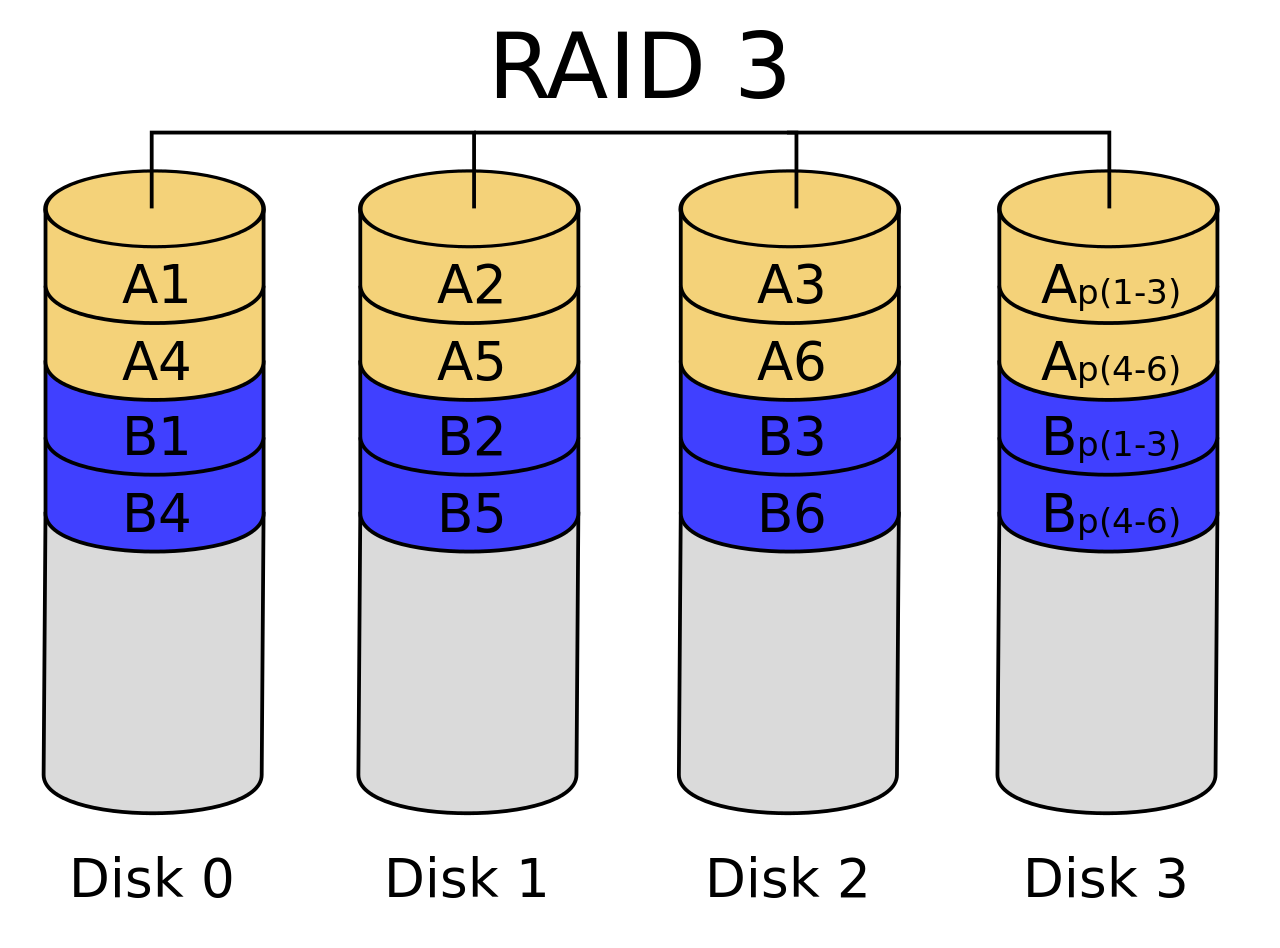
\includegraphics[clip,width=10.0cm]{images/RAID_3.png}
				\caption{Diagrama do RAID 3. }
				\label{fig:raid3}
			\end{center}
		\end{figure} 
		
		\subsubsection{Desempenho}
		Esta configuração se encaixa para aplicações que necessitam de altas taxas de transferência de grandes sequências de dados sequenciais, como por exemplo, edição de vídeos não compressados. Todavia, aplicações que fazem uso de leituras e escritas em localizações aleatórias do disco tendem a ter um desempenho inferior, visto que as frações de um mesmo dado estão espalhadas nas mesmas seções dos vários discos do vetor.\\
		
		\subsection{RAID 4}
		Diferente dos RAID 2 e 3, o RAID 4 fraciona os dados ao nível do bloco de dados, tendo um disco dedicado de paridade. \\
		
		A figura ~\ref{fig:raid4} representa o diagrama de um vetor modelado com o RAID 4 utilizando-se quatro discos, sendo um deles utilizados como disco de paridade.\\
		
		\begin{figure}[htb]
			\begin{center}
				
				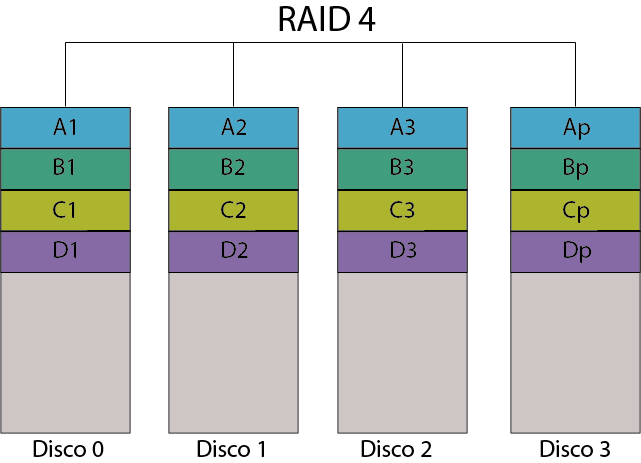
\includegraphics[clip,width=10.0cm]{images/RAID_4.png}
				\caption{Diagrama do RAID 4. }
				\label{fig:raid4}
			\end{center}
		\end{figure} 
		
		\subsubsection{Desempenho}
		Sempre que os dados são escritos no vetor, o novo dado sobre paridade deve ser recalculado e escrito para o respectivo disco de paridade antes que qualquer requisição de escrita seja realizada. Por causa dessas operações de leitura e escrita, o disco de paridade é o fator limitante do desempenho total do vetor.\\
		
		\subsection{RAID 5}
		Similar ao RAID 4, o RAID 5 fraciona os dados ao nível do bloco de dados, porém tendo as informações de paridade espalhadas entre os discos do vetor. Isto exige que todos, exceto um, discos tenham os dados. No caso da falha de apenas um disco, leituras subsequentes podem ser calculadas utilizando-se os dados restantes e (caso o disco defeituoso não seja o que continha os dados de paridade do arquivo) das informações de paridade para recuperar o bloco faltoso de dados. Entretanto, caso o disco que está indisponível é o portador dos dados de paridade, não acarreta na necessidade de nenhum calculo a mais. É importante frisar que por suas características, o RAID 5 necessita de ao menos três discos.  \\
		
		A figura ~\ref{fig:raid5} representa o diagrama de um vetor modelado com o RAID 5 utilizando-se quatro discos.\\
		
		\begin{figure}[htb]
			\begin{center}
				
				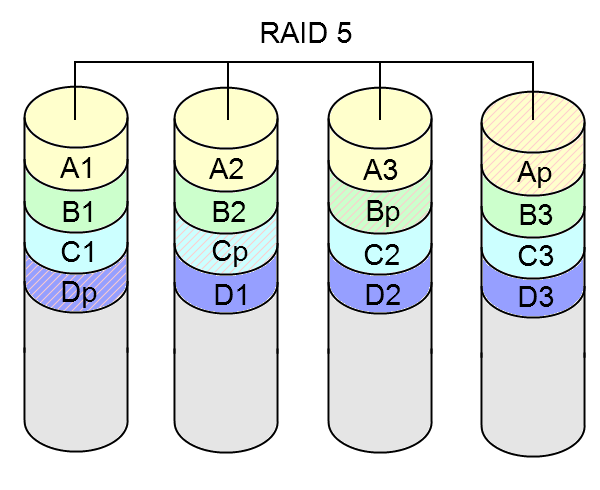
\includegraphics[clip,width=10.0cm]{images/RAID_5.png}
				\caption{Diagrama do RAID 5. }
				\label{fig:raid5}
			\end{center}
		\end{figure} 
		
		\subsubsection{Desempenho}
		O RAID 5 sofre pelo tempo demasiadamente grande necessário para reconstruir um arquivo a partir dos blocos restantes e do bloco de paridade, além da chance de mais de um disco ficar indisponível durante a fase de recuperação. Como a recuperação de um bloco de dados requer a leitura de todos os blocos de dados, abre-se a chance de perder todos os dados do vetor caso ocorra a perda de um segundo disco.\\
		
		\subsection{RAID 6}
		Similar ao RAID 5, o RAID 6 fraciona os dados em nível do bloco de dados, porém tendo as informações de paridade espalhadas entre os discos do vetor e duplicadas. A novidade da paridade dupla garante tolerância a falhas até o caso da perda de dois discos. RAID 6 exige a utilização de no mínimo quatro discos. \\ 
		
		Semelhante ao caso do RAID 5, a queda de um disco acarreta na redução do desempenho de todo o vetor até que o disco defeituoso tenha sido substituído.\\

		
		A figura ~\ref{fig:raid6} representa o diagrama de um vetor modelado com o RAID 6 utilizando-se cinco discos.\\
		
		\begin{figure}[htb]
			\begin{center}
				
				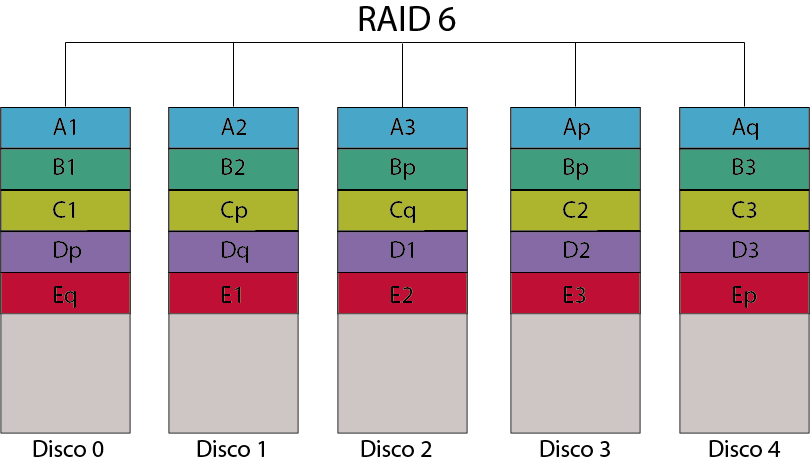
\includegraphics[clip,width=10.0cm]{images/RAID_6.png}
				\caption{Diagrama do RAID 6. }
				\label{fig:raid6}
			\end{center}
		\end{figure} 
		
		\subsubsection{Desempenho}
		RAID 6 não possui penalidade de desempenho sobre operações de leitura, contudo, possui penalidade de desempenho nas operações de escrita devido ao \textit{overhead} associado aos cálculos de paridade.\\
		
		
		\subsection{RAID 50}
		Existe o termo originalmente conhecido como RAID híbrido, o qual é definido pela aplicação de um nível de RAID sobre outro vetor formado por nível de RAID. O último vetor gerado é conhecido como o 
		vetor do topo. Logo, no caso do RAID 50 (ou RAID 5+0) é uma combinação híbrida que usa as técnicas de RAID 5 com paridade em conjunção com a segmentação de dados do RAID 0. Em outras palavras, o RAID 50 não passa da aplicação do RAID 0 sobre um vetor de RAID 5. \\
		
		A figura ~\ref{fig:raid50} representa o diagrama de um vetor modelado com o RAID 50 utilizando-se três conjuntos de três discos cada.\\
		
		\begin{figure}[htb]
			\begin{center}
				
				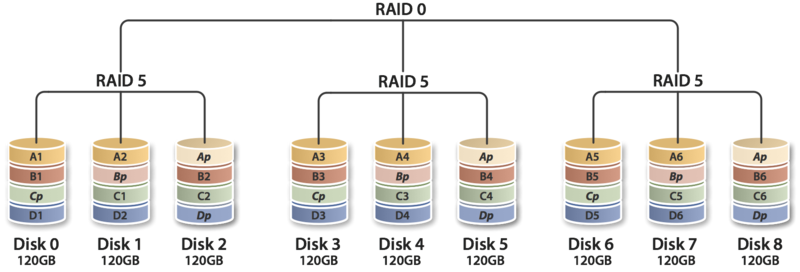
\includegraphics[clip,width=15.0cm]{images/RAID_50.png}
				\caption{Diagrama do RAID 50. }
				\label{fig:raid50}
			\end{center}
		\end{figure} 
		
		\subsubsection{Desempenho}
		Possui alta taxa de transferência, porém com alto custo de manutenção e expansão.
		
	%texto.... referência~\citep{patterson88}
	
	\section{Conclusões do Capítulo}
	Neste capítulo foi apresentado os conceitos de básicos do que é RAID, suas características positivas e negativas, além de abordar sobre as topologias mais importantes do RAID, ou seja, RAID 0, RAID 1, RAID 2, RAID 3, RAID 4, RAID 5, RAID 6 e RAID 50.
	Vale destacar que ainda existem outros tipos de RAID oriundo de combinação destes tipos apresentados.
		



 

	

